\documentclass[11pt,border=0mm,tikz]{standalone}
\usepackage{csquotes}
\usepackage[backend=biber,style=numeric,sorting=none]{biblatex}

% ===================== Figure size & fonts =========================
% Include at NATURAL size: \includestandalone WITHOUT width=..., so one
% drawing unit equals one document unit and every label is set at the
% 11pt body sizes (\small, \footnotesize, ... then match the running
% text exactly; the 11pt class option above sets that baseline).
% Need it smaller? Lower \FigScale -- as this diagram is built from
% fixed-size boxes it zooms uniformly (geometry AND fonts together), so
% \FigScale=1 keeps the labels at body size. Do NOT pass width= to the
% include: that magnifies the text together with the picture.
% ===================================================================
\providecommand{\FigScale}{1}
\usepackage{siunitx}
\usepackage{tikz}
\usetikzlibrary{decorations.pathmorphing,patterns}
\usetikzlibrary{shapes.geometric, arrows.meta}
\usetikzlibrary{positioning}
\usepackage{amsmath}
\usepackage{upgreek}
\usepackage{svg}
\usetikzlibrary{3d}
\usetikzlibrary{calc}
\tikzset{
box/.style={
	rectangle,
	rounded corners=4pt,
	minimum width=3cm,
	minimum height=1cm,
	text centered,
    align=center,
	draw=black!70,
	line width=0.95pt,
	fill=gray!5,
	inner sep=4pt
},
decision/.style={
	diamond,
	aspect=2,
	text centered,
	align=center,
	draw=black!70,
	line width=0.95pt,
	fill=gray!5,
	inner sep=1pt
},
arrow/.style={
	thick,
	->,
	>=Stealth,
	draw=black!70,
	line width=1pt,
	line cap=round,
	line join=round,
	shorten <=1pt,
	shorten >=1pt
}
}
\begin{document}
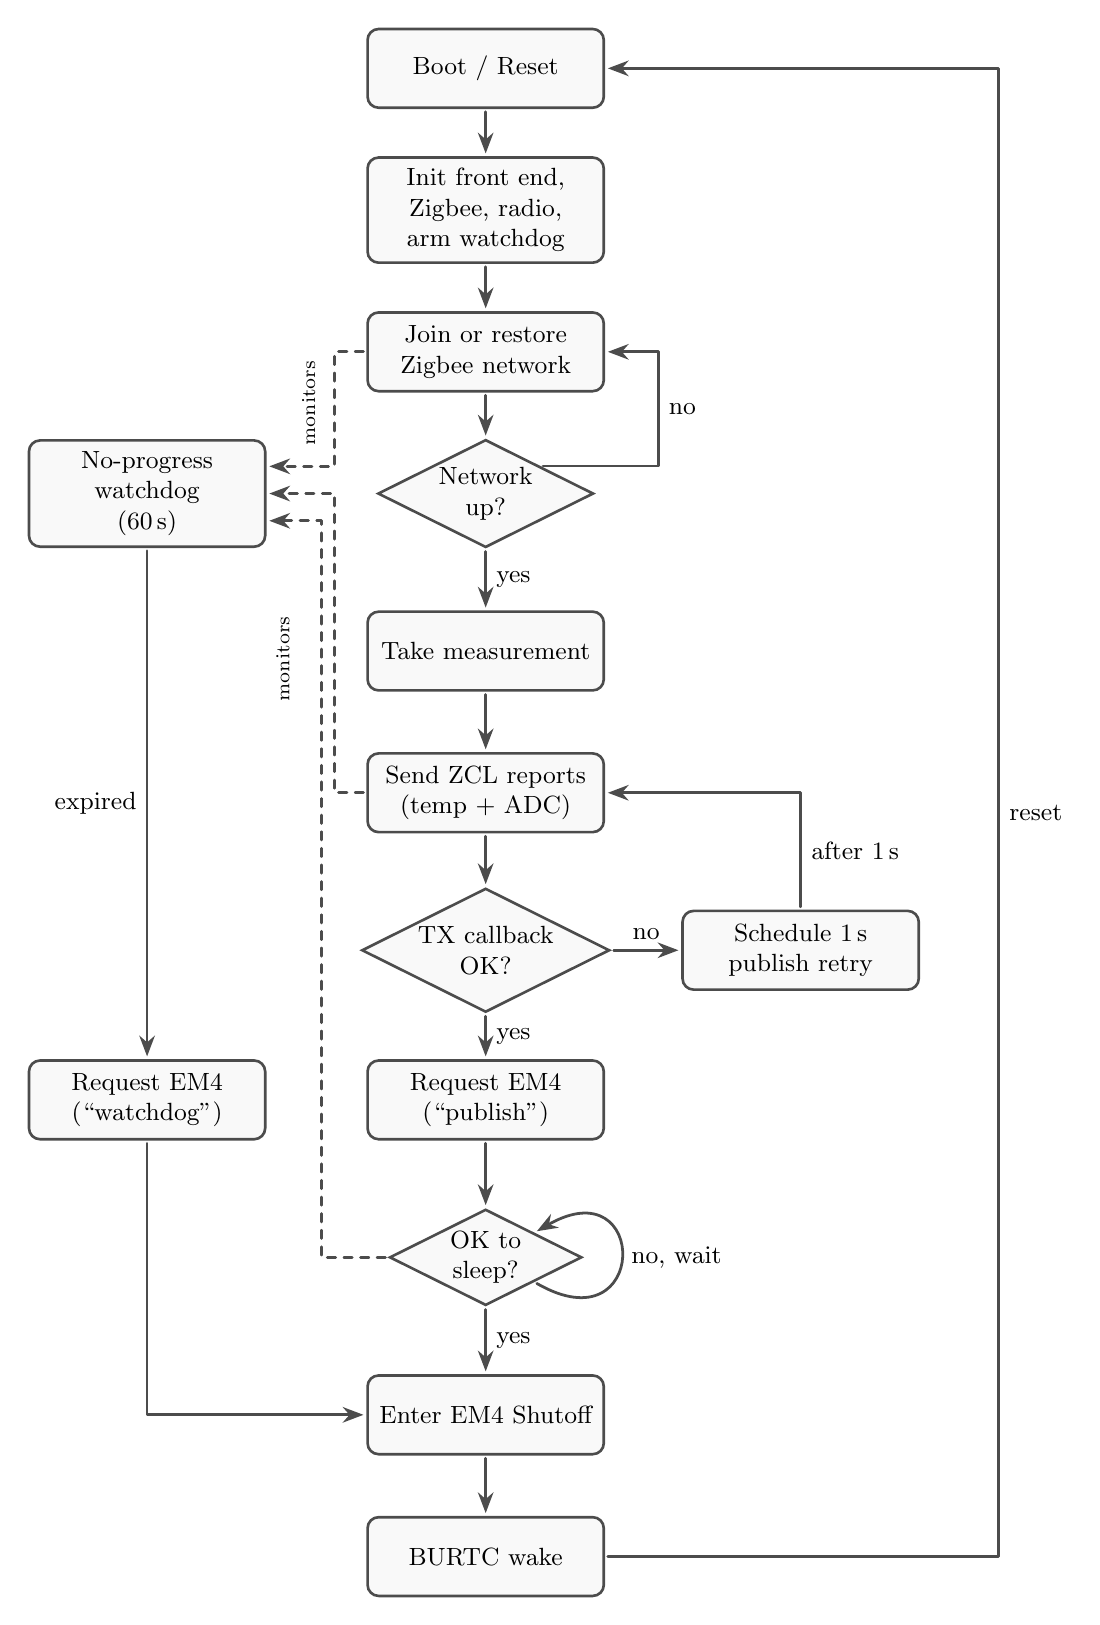
\begin{tikzpicture}[font=\small, scale=\FigScale, transform shape]
% ===== Main vertical happy path (centre column, x = 0) =====
\node (boot)    [box]                         at (0, 0)    {Boot / Reset};
\node (init)    [box]                         at (0, -1.8) {Init front end,\\Zigbee, radio,\\arm watchdog};
\node (join)    [box]                         at (0, -3.6) {Join or restore\\Zigbee network};
\node (upq)     [decision]                    at (0, -5.4) {Network\\up?};
\node (measure) [box]                         at (0, -7.4) {Take measurement};
\node (report)  [box]                         at (0, -9.2) {Send ZCL reports\\(temp + ADC)};
\node (txq)     [decision]                    at (0, -11.2){TX callback\\OK?};
\node (em4req)  [box]                         at (0, -13.1){Request EM4\\(``publish'')};
\node (okq)     [decision]                    at (0, -15.1){OK to\\sleep?};
\node (em4)     [box]                         at (0, -17.1){Enter EM4 Shutoff};
\node (wake)    [box]                         at (0, -18.9){BURTC wake};
% ===== Side nodes =====
% TX failure -> retry (right side)
\node (retry)   [box]                         at (4.0, -11.2){Schedule 1\,s\\publish retry};
% Watchdog (left side)
\node (wdog)    [box]                         at (-4.3, -5.4){No-progress\\watchdog\\(60\,s)};
\node (em4w)    [box]                         at (-4.3, -13.1){Request EM4\\(``watchdog'')};
% ===== Happy-path arrows =====
\draw [arrow] (boot)    -- (init);
\draw [arrow] (init)    -- (join);
\draw [arrow] (join)    -- (upq);
\draw [arrow] (upq)     -- node[right] {yes} (measure);
\draw [arrow] (measure) -- (report);
\draw [arrow] (report)  -- (txq);
\draw [arrow] (txq)     -- node[right] {yes} (em4req);
\draw [arrow] (em4req)  -- (okq);
\draw [arrow] (okq)     -- node[right] {yes} (em4);
\draw [arrow] (em4)     -- (wake);

% wake -> boot (full reset), routed on the far right
\draw [arrow] (wake.east) -- ++(5.0,0) |- node[pos=0.25, right] {reset} (boot.east);
% Network not up: wait (loop back into join from the right side)
\draw [arrow] (upq.north east) -- ++(1.5,0.0) |- node[pos=0.25, right] {no} (join.east);
% OK to sleep? no -> wait (circular self-loop back into the decision)
\draw [arrow] (okq.south east) to[out=-30, in=30, looseness=6.9]
      node[pos=0.5, right] {no, wait} (okq.north east);
% TX failure -> retry -> back to report after 1 s
\draw [arrow] (txq.east)   -- node[above] {no} (retry.west);
\draw [arrow] (retry.north) |- node[pos=0.25, right] {after 1\,s} (report.east);
% Watchdog: stuck anywhere in active phase -> request EM4 (watchdog) -> EM4
\draw [arrow] (wdog) -- node[left] {expired} (em4w);
\draw [arrow] (em4w.south) |- (em4.west);

\draw [arrow, dashed] (join.west)   -- ++(-0.4,0)
      |- ($(wdog.east)!0.5!(wdog.north east)$);
\draw [arrow, dashed] (report.west) -- ++(-0.4,0)
      |- (wdog.east);
\draw [arrow, dashed] (okq.west)    -- ++(-0.85,0)
      |- ($(wdog.east)!0.5!(wdog.south east)$);

\node[font=\scriptsize, rotate=90] (monlbl) at (-2.25,-4.25) {monitors};
\node[font=\scriptsize, rotate=90] (monlbl) at (-2.575,-7.5) {monitors};

\end{tikzpicture}
\end{document}